%!TEX TS-program = xelatex
%!TEX encoding = UTF-8 Unicode

\documentclass[11pt]{article}
\usepackage[utf8]{inputenc}
\usepackage{xunicode,xltxtra, polyglossia}
\usepackage{fontspec} %(include if mathspec is not loaded)
\usepackage[a4paper, margin = 1 in, left = .5 in, right = .5 in]{geometry}

\usepackage[dvipsnames]{xcolor}
\usepackage{enumitem}
\usepackage{amsmath}
\usepackage{amssymb}
\usepackage{tikz}

\usepackage{fancyhdr}
\pagestyle{fancy}

\usepackage{linguex}
\usepackage{multicol}

\usepackage[colorlinks, hyperfootnotes=false]{hyperref} % hyperlinks
\hypersetup{linkcolor=MidnightBlue,citecolor=MidnightBlue,filecolor=MidnightBlue,urlcolor=MidnightBlue} 

\usepackage{pifont}% http://ctan.org/pkg/pifont
\newcommand{\cmark}{\ding{51}}%
\newcommand{\xmark}{\ding{55}}%

\lhead{\opt \Large GPP  experiments notes}
\rhead{\opt \large Lisa Hofmann\\ \today}
\cfoot{\thepage}


%language
\setdefaultlanguage[variant=american]{english}
% \def\hyph{-\penalty0\hskip0pt\relax}

% fonts
\defaultfontfeatures{Mapping=tex-text, Ligatures=TeX}
\setromanfont[Mapping=tex-text, Numbers={Proportional}]{Linux Libertine}
\setsansfont[Scale=MatchLowercase,Mapping=tex-text]{Optima}
% \setmonofont[Scale=MatchLowercase]{Andale Mono}
\newfontfamily\opt{Optima}


\begin{document}
\tableofcontents

% \section{Questions} % (fold)
% 	\begin{itemize}
% 		\item Were the questions for projection / at-issueness diagnostics asked in randomized order?
% 		\item What were the thoughts on arousal? How would this come into play? Is the idea that it would interact with the QUD?
% 		\item How exactly are the pilots different from the main experiments?
% 	\end{itemize}

% % section questions (end)

\pagebreak
\section{Experiments with Declaratives and Negation}

	\paragraph{Summary} % (fold)

		\begin{itemize}
			\item We don't see the correlation between non-at-issueness measures and projection measures here that are predicted by the GPP
			\item This seems to be due to problems with the intended at-issueness diagnostics: They confound at-issueness with speaker commitments, which does make them sensitive to projection as well
		\end{itemize}

	% paragraph summary (end)

	\subsection{2n---Negation embedding, yes, that's true+complement diagnostic (+ acceptability rating)}
			\ex. \a. \textbf{Christopher:} Cole didn’t discover that Julian dances salsa.
				\b. \textbf{Sandy:} Yes, that’s true, Julian dances salsa.
				\z.
			\z.

			\begin{itemize}
				
				\item yes, that's true+complement diagnostic for at-issueness (?):
				\begin{itemize}
					\item Tests whether you can agree with the previous assertion and assert the complement
					\item so, in a sense this is a diagnostic of projection as well
				\end{itemize}
				

				\item Certain-that diagnostic for projection: Tests whether participant assumes that speaker is committed to complement

				\item Projection does not correlate with the (intended) non-at-issueness measures
			\end{itemize}

			\begin{figure}[h]
				\centering
				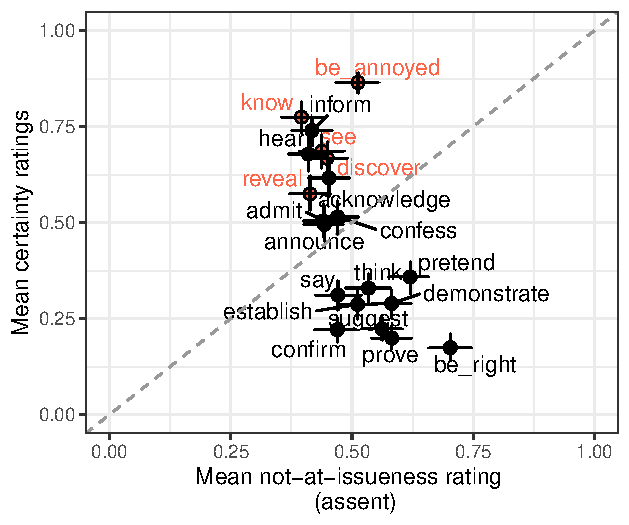
\includegraphics[]{figures/n2-correl.pdf}
				\caption{Mean not-at-issueness ratings vs mean certainty ratings by predicate, Exp. 2n}
				\label{fig:figure1}
			\end{figure}

			\begin{itemize}
				\item In fact, it looks like there might be an inverse relationship
				\item I would expect that projection-measure correlates better with the opposite (i.e. the intended measure of at-issueness)
				\item For declaratives, a different at-issueness diagnostic may be needed
				
			\end{itemize}

	\subsection{How does the correlation for 2n look for projection vs. the positive responses to the assent-diagnostic?} % (fold)	
		Plot for correlation between projectivity-measure and high acceptability ratings for assent w/ assertion of complement.

			\begin{figure}[h]
				\centering
				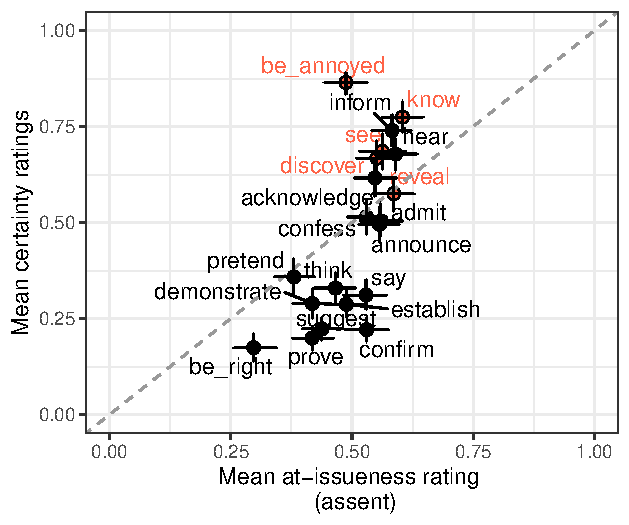
\includegraphics[]{figures/n2-inv-correl.pdf}
				\caption{Mean at-issueness ratings vs mean certainty ratings by predicate, Exp. 2n}
				\label{fig:figure4}
			\end{figure}


		\begin{itemize}
			\item This looks more like a non-linear correlation
		\end{itemize}
	% subsection how_does_the_correlation_for_2n_look_with_at_issueness_ (end)

	\subsection{3n---Negation embedding, yes, that's true + negation of main clause (+ acceptability rating)} % (fold)
		\ex. \a. \textbf{Christopher:} Cole didn’t discover that Julian dances salsa.
				\b. \textbf{Sandy:} Yes, that’s true, but Cole discovered it.
				\z.
			\z.

			\begin{itemize}
				
				\item yes, that's true+negation of main clause diagnostic for at-issueness:
				\begin{itemize}
					\item Tests whether you can agree with the previous assertion and assert the negation of the main clause
					\item agreement with main point of previous utterance
					\item If the main point was the complement, and the first speaker is committed to truth of the complement, then assent should be possible while rejecting the main clause.
					\item This addresses at-issueness of the complement.
					\item But potentially also confounds speaker commitment to complement (i.e. projection) with at-issueness.
					\item This is assuming that assent signals that the second speaker takes on (some of) the commitments of the first speaker.
					\item Based on this assumption, we can also assume the acceptability ratings to be relatively low throughout. %(see \textbf{Figure \ref{fig:figure5}})
				\end{itemize}

				% \begin{figure}[h]
				% 	\centering
				% 	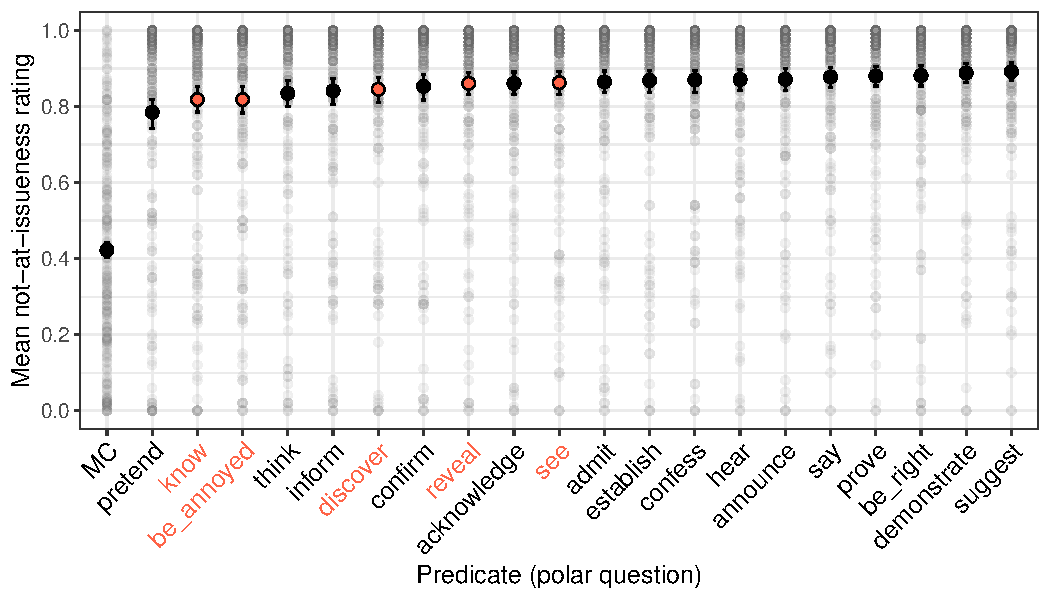
\includegraphics[width=.75\textwidth]{figures/n3-nai.pdf}
				% 	\caption{Mean not-at-issueness ratings by predicate, Exp. 3n}
				% 	\label{fig:figure5}
				% \end{figure}
				
				% \pagebreak
				\item Certain-that diagnostic for projection: Tests whether participant assumes that speaker is committed to complement

				\item Does projection correlate with the (intended) non-at-issueness measures? If there is a confound, we would again expect something more to the opposite effect. (see \textbf{Figure \ref{fig:figure6}})
			\end{itemize}

			\begin{figure}[h]
				\centering
				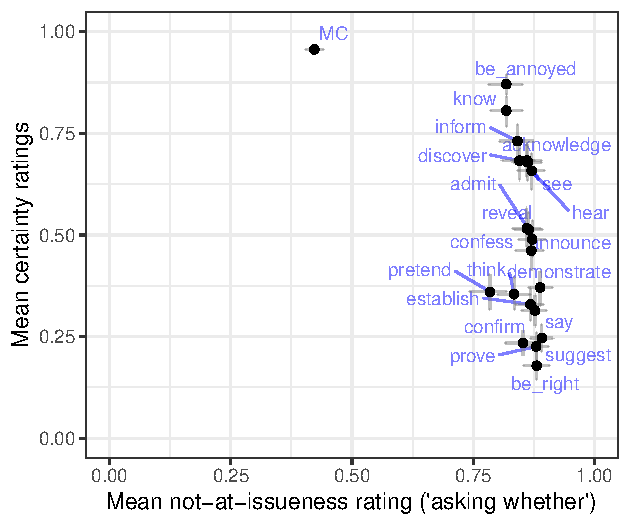
\includegraphics[scale=0.90]{figures/n3-correl.pdf}
				\caption{Mean not-at-issueness ratings vs mean certainty ratings by predicate, Exp. 3n}
				\label{fig:figure6}
			\end{figure}

	% subsection 3n_negation_embedding_yes_that_s_true_negation_of_main_clause_acceptability_rating (end)

	\pagebreak
	\subsection{1n---Negation embedding, are you sure?, assent + assertion of complement + Q-A judgment} % (fold)
		\ex. \a. \textbf{Christopher:} Cole didn’t discover that Julian dances salsa.
				\b. \textbf{Sandy:} Are you sure?
				\b. \textbf{Christopher:} Yes, I'm sure that Julian dances Salsa.
				\z.
			\z.

		\begin{itemize}
			\item This diagnostic also conflates non-at-issueness with projection: Only if Christopher is committed to truth of the complement can they respond in this way 

			\item Here, also we don't see the correlation come out (\textbf{Figure \ref{fig:1n-correl}})
		\end{itemize}

			\begin{figure}[h]
					\centering
					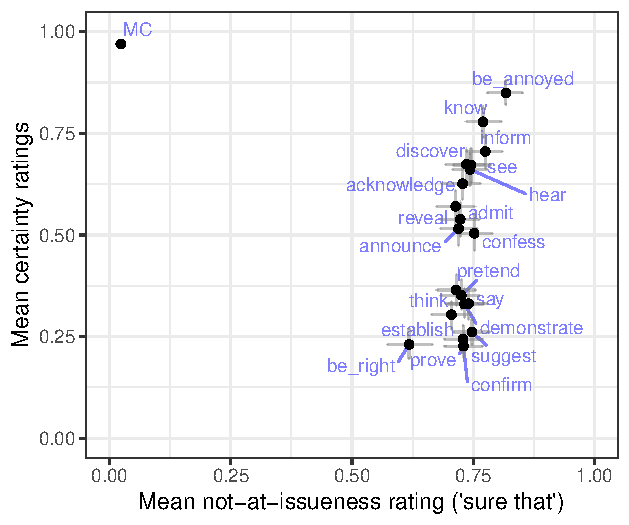
\includegraphics[scale=0.9]{figures/n1-correl.pdf}
					\caption{Mean at-issueness ratings vs mean certainty ratings by predicate, Exp. 1n \label{fig:1n-correl}}
				\end{figure}

	% subsection 1n_negation_embedding_are_you_sure_q_a_judgment (end)

	\pagebreak
	\subsection{A conclusion about at-issueness diagnostics} % (fold)
		\begin{itemize}
			\item A diagnostic of at-issueness should not interact with speaker commitment
			\item Problem with negation: If the complement is at issue, it will be targeted by entailment-cancelling operators
			\item On the other hand, if the complement is not at issue, it is predicted to project
			\item A diagnostic should target the question of whether the first utterance addresses the quesion $\{c, \neg c\}$, while leaving open how exactly the question is resolved

			\item Here is one idea:
		\end{itemize}
	
		\begin{itemize}
			\item Asking what it was about without commitment:
				\ex. \a. \textbf{Christopher:} Cole didn’t discover that Julian dances salsa.
					\b. \textbf{Sandy:} Oh right, Mary told me that as well.\\
					\textbf{Forced Choice:} What did Mary talk to Sandy about?
						\a. Whether Julian dances salsa.
						\b. Whether Cole discovered that Julian dances salsa.
						\z.
					\z.
				\z.

			% \pagebreak
			\item Question-answer based: Can the declarative address a question about the complement?
				\ex. \a. \textbf{Sandy:} Does Julian dance salsa?
					\b. \textbf{Christopher:} Cole didn’t discover that Julian dances salsa.\\
						\textbf{Q-A judgment:} Did Christopher answer Sandy's question?
					\z.
				\z. 

			\item Anaphora-based:

				\ex. \a. \textbf{Christopher:} Cole didn’t discover that Julian dances salsa.
					\b. \textbf{Sandy:} That would be quite surprising.\\
					\textbf{Forced Choice:} What would Sandy find surprising?
						\a. Julian dancing salsa.
						\b. Cole discovering that Julian dances salsa.
						\z.
					\z.
				\z.

		\end{itemize}

		\noindent These tests separate at-issueness diagnostics from commitment, as well as the question of whether or not the second speaker (dis)agrees with the first.
		
		\begin{itemize}
			\item This is important, especially under negation, because if we expect that at-issueness correlates with non-projection, we expect the complement to be targeted by negation, and therefore counterfactual.

			\item Separating at-issueness and commitment of the complement I think that we can expect a correlation between non-at-issueness and projection again.
				
				\ex. \textbf{Context:} Cole is a child that is being picked up from daycare
					\a. \textbf{Parent:} What did Cole do today?
					\b. \textbf{Caretaker:} Cole didn't see that Julian danced salsa.\\
					$\Rightarrow$ Probable inference that Julian danced salsa
					\z.
				\z.

				\ex. \textbf{Context:} Julian is a child that is being picked up from daycare 
					\a. \textbf{Parent:} What did Julian do today?
					\b. \textbf{Caretaker:} Cole didn't see that Julian danced salsa.\\
					$\Rightarrow$ Probable inference that Julian did not dance salsa (?)\\
					$\Rightarrow$ Additional evidential inference Cole is a reliable source on whether Julian danced Salsa
					\z.
				\z.

			\item That should be the case, at least for certain predicates, namely veridical ones (see discussion below)

			\item Some open questions:
			\begin{itemize}
				\item The experiment assumes that the probability of complement at-issueness is influenced by the lexical embedding. That seems to be the case

				\item However, there are other factors that can influence at-issueness
				\begin{itemize}
					\item \textbf{Discourse context (QUD):} An utterance is more likely to be about a topic that has already been brought up/a question that has been raised
					\item \textbf{Epistemic context (common ground):} An utterance is more likely to be about an issue that hasn't been settled
				\end{itemize}

			\end{itemize}

		\end{itemize}

	
	% subsubsection a_conclusion_about_at_issueness_diagnostics (end)

% \pagebreak
\section{Experiments with question embedding} % (fold)

	\paragraph{Summary} % (fold)
		\begin{itemize}
			\item For questions, the correlation comes out more clearly
			\item This suggests that the at-issueness diagnostics for questions work better.
				\begin{itemize}
					\item This seems clear for asking-whether diagnostic
					\item Although we questioned this last time, I think that it applies to yes+$c$ diagnostic
					\item It doesn't work for yes but not $c^\prime$ diagnostic
				\end{itemize}

			\item There are some lexical exceptions wrt the correlation
			\item The exceptions are:
			\begin{itemize}
				\item Mostly non-veridical predicates (\emph{say, suggest, think, pretend})
					\begin{itemize}
						\item This suggests lexical contibution of the verb:
						\item Only if the verb is associated with an inference about the truth of the complement, that inference can project
					\end{itemize}
					

				\item Maybe some veridical assertives(?) (\emph{prove, \textcolor{gray!50}{establish, demonstrate, confirm}})
				\begin{itemize}
					\item c.f. Anand \& Hacquard 2014 on epistemic vs assertive attitudes: veridical epistemics are factive, while veridical assertives are non-presuppositional
					\item Interestingly, though, other veridical assertives behave differently (\emph{inform, acknowledge, confess, admit})
					\item Not sure if the latter group actually is characterized as in the same way in A\&H: do they take (non-agentive/non-intentional) repository of information subjects (e.g. \emph{\#/? The test results informed us/ acknowledged/confessed/admitted that Mary is free of contagious diseases.} vs. \emph{The test results proved/ established/demonstrated/confirmed that Mary is free of contagious diseases.})
					\item These two groups are discussed in A\&H as apparent counterexamples
					\item Djärv (2019): analysis of non-projection as involving evidential interpretations
				\end{itemize}
			\end{itemize}
		\end{itemize}
	
	% paragraph summary (end)
		
	\pagebreak
	\subsection{1q---Question embedding, asking-whether diagnostic} % (fold)
			
			\ex. \a. \textbf{Christopher:} Did Cole discover that Julian dances salsa?
				\b. \textbf{Question-based at-issueness diagnostic:} Is Christopher asking whether Julian dances salsa?
				\z.
			\z.

			\begin{itemize}
				
				\item Asking-whether diagnostic for at-issueness:
				\begin{itemize}
					\item Tests whether the utterance is \lq about\rq\ the truth of the complement
					\item Question-based at-issueness diagnostic
					\item What is the main point of the utterance?
				\end{itemize}
				

				\item Certain-that diagnostic for projection: Tests whether participant assumes that speaker is committed to complement

				\item Not-at-issueness correlates with projection (\textbf{Figure \ref{fig:q1-correl}})
				\begin{itemize}
					\item but only for veridical predicates
					\item the lexical exceptions are non-veridical predicates
					\item Updated GPP (?): given an inference is associated with a predicate, it will project to the extent that it is not at issue
				\end{itemize}

			\end{itemize}

			\begin{figure}[h]
				\centering
				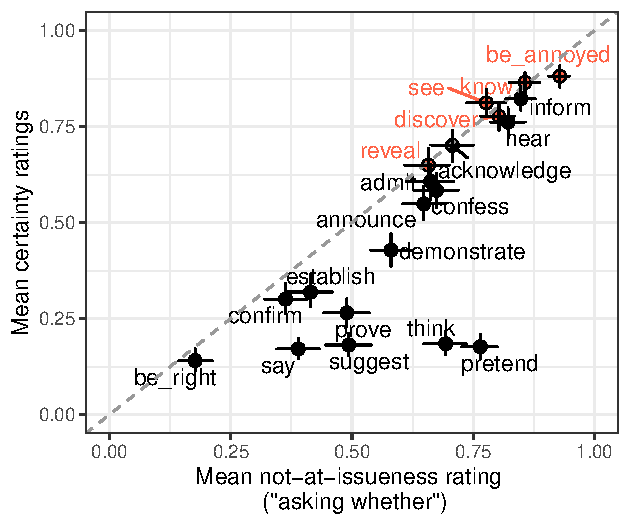
\includegraphics[]{figures/q1-correl.pdf}
				\caption{Mean not-at-issueness ratings vs mean certainty ratings by predicate, Exp. 1q}
				\label{fig:q1-correl}
			\end{figure}

	% subsection q1_question_embedding_asking_whether_diagnostic (end)

	\pagebreak
	\subsection{2q---Question embedding, yes+complement diagnostic (+ acceptability rating)} % (fold)
		\ex. \a. \textbf{Christopher:} Did Cole discover that Julian dances salsa?
				\b. \textbf{Sandy:} Yes, Julian dances salsa.
				\z.
			\z.

			\begin{itemize}
				\item yes+c diagnostic for at-issueness (acceptablity rating):
				\begin{itemize}
					\item Tests whether an affirmative response to the question can be accompanied with an assertion of the complement (there is an intuitive sense in which they should be \lq about\rq\ the same thing)

					\item Therefore, this can also be understood as a diagnostic of the main point of the question

				\end{itemize}
				

				\item Certain-that diagnostic for projection: Tests whether participant assumes that speaker is committed to complement

				\item Not-at-issueness correlates with projection (\textbf{Figure \ref{fig:q2-correl}})
				\begin{itemize}
					\item Similar pattern of lexical exceptions
					\item They are more spaced out here
				\end{itemize}
			\end{itemize}

			\begin{figure}[h]
				\centering
				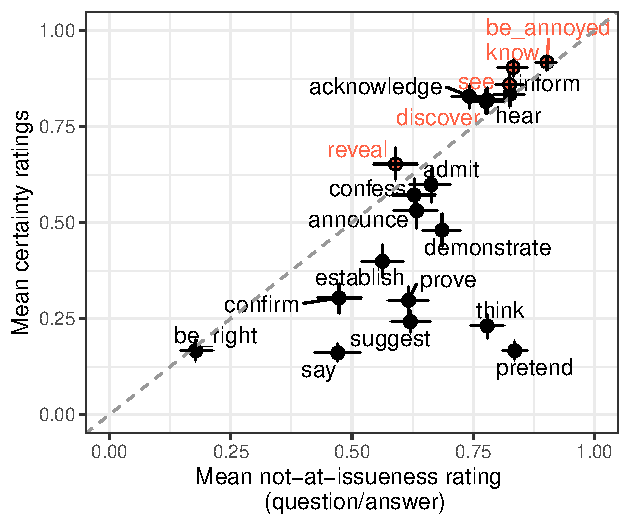
\includegraphics[]{figures/q2-correl.pdf}
				\caption{Mean not-at-issueness ratings vs mean certainty ratings by predicate, Exp. 2q}
				\label{fig:q2-correl}
			\end{figure}
		
	% subsection q1_question_embedding_asking_whether_diagnostic (end)

	\subsection{3q---Question embedding, yes but not $c^\prime$ (+ acceptability rating)}
		\ex. \a. \textbf{Christopher:} Did Cole discover that Julian dances salsa?
				\b. \textbf{Sandy:} Yes, Julian dances salsa.
				\z.
			\z.

		\begin{itemize}
				\item yes but not $c^\prime$ diagnostic for at-issueness (acceptablity rating):
				\begin{itemize}
					\item Tests whether an affirmative response to the question can be accompanied with a denial of the main clause

					\item Expectation: If the question is about the complement, we might be able to affirm the complement while denying the main clause

					\item This is, again, based on the assumption that the complement and main clause are interpreted independent of each other

					\item However, if Djärv (2019) is right that projective interpretations are interpreted as evidentials, it is expected that we cannot affirm the complement while rejecting the main clause, in cases where there is projection.

					\item In fact all ratings for this test are quite low overall.

				\end{itemize}
				

				\item Certain-that diagnostic for projection: Tests whether participant assumes that speaker is committed to complement

				\item (Intended) not-at-issueness measure does not correlate with projection, see \textbf{Figure \ref{fig:q3-correl}}
			\end{itemize}

			\begin{figure}[h]
				\centering
				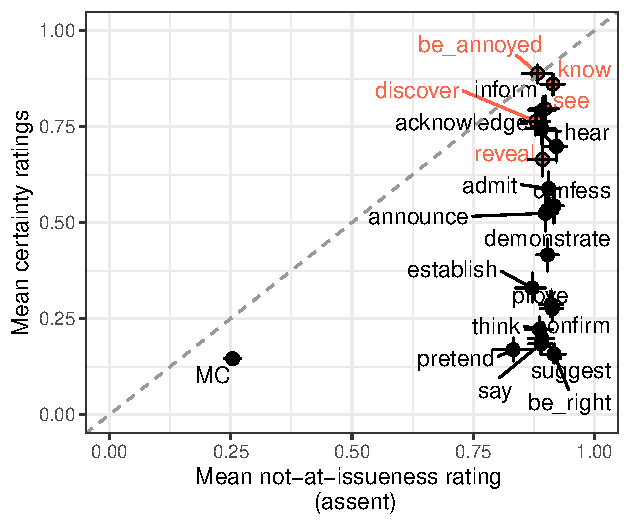
\includegraphics[]{figures/q3-correl.pdf}
				\caption{Mean not-at-issueness ratings vs mean certainty ratings by predicate, Exp. 3q
				\label{fig:q3-correl}}
			\end{figure}

	% subsection

% section three_experiment_setups (end)


\section{Experiments with modals}
	\subsection{1m---Modal embedding (perhaps),  are you sure?, assent + assertion of complement + Q-A judgment} % (fold)
		\ex. \a. \textbf{Christopher:} Perhaps Cole discovered that Julian dances salsa.
			\b. \textbf{Sandy:} Are you sure?
			\b. \textbf{Christopher:} Yes, I'm sure that Julian dances Salsa.
			\z.
		\z.

		\begin{itemize}
			\item Like with negation above, this test clearly conflates at-issueness and projection: Only of Christopher is committed to $c$, can they respond in this way
			
			\item Correlation does not exactly come out see \textbf{Figure \ref{fig:m1-corr}}
			\begin{itemize}
				\item However, more so than for negation
				\item Interestingly, the lexical exceptions are similar here: \emph{prove, say, suggest, think, pretend}
			\end{itemize}
		\end{itemize}

		\begin{figure}[h]
			\centering
			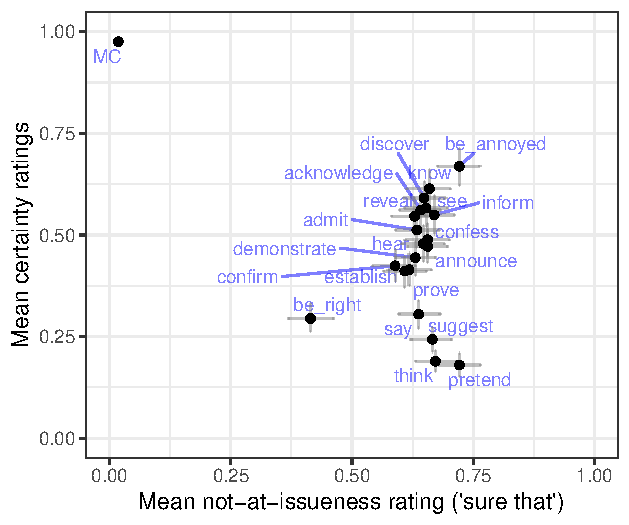
\includegraphics[scale=0.85]{figures/m1-correl.pdf}
			\caption{Mean not-at-issueness ratings vs mean certainty ratings by predicate, Exp. 1m}
			\label{fig:m1-corr}
		\end{figure}
	
	% subsection 1m_modal_embedding_ (end)

	\pagebreak
	\subsection{2m---Modal embedding (perhaps) yes, that's true+complement diagnostic (+ acceptability rating)} % (fold)
		\ex. \a. \textbf{Christopher:} Perhaps Cole discovered that Julian dances salsa.
			\b. \textbf{Sandy:} Yes, that’s true, Julian dances salsa.
			\z.
		\z.

		\begin{itemize}
			\item Same test as above: Intended at-issueness measure also tests whether agreeing is possible while asserting the complement: confound with commitment

			\item Overall acceptabiliy ratings are higher for this test compared to 1m
			
			\item But the overall pattern in correlation with projection-measure is similar \textbf{Figure \ref{fig:m2-corr}}
			\begin{itemize}
				\item More of a correlation compared to negation experiments
				\item Again same predicates outside of the main cluster: \emph{prove, say, suggest, think, pretend}
			\end{itemize}
		\end{itemize}

		\begin{figure}[h]
			\centering
			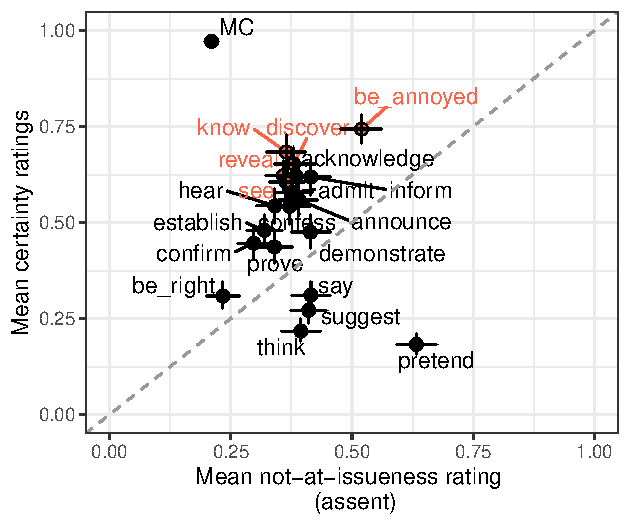
\includegraphics[scale=0.85]{figures/m2-correl.pdf}
			\caption{Mean not-at-issueness ratings vs mean certainty ratings by predicate, Exp. 2m}
			\label{fig:m2-corr}
		\end{figure}
	
	% subsection 1m_modal_embedding_ (end)

	\pagebreak
	\subsection{3m---Modal embedding (perhaps), yes, that's true + negation of main clause (+ acceptability rating)} % (fold)
		\ex. \a. \textbf{Christopher:} Perhaps Cole discovered that Julian dances salsa.
			\b. \textbf{Sandy:} Yes, that’s true, but Cole didn't discover it.
			\z.
		\z.

		\begin{itemize}
			\item Similar pattern to other modal experiments above
		\end{itemize}

		\begin{figure}[h]
			\centering
			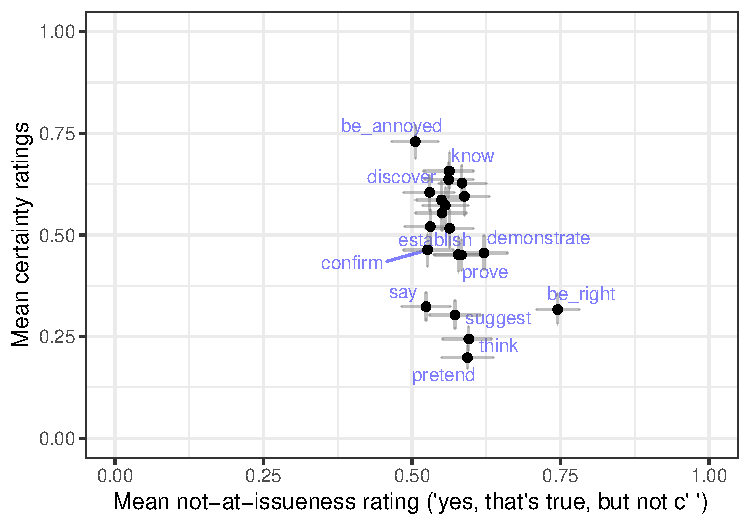
\includegraphics[]{figures/m3-correl.pdf}
			\caption{Mean not-at-issueness ratings vs mean certainty ratings by predicate, Exp. 3m}
			\label{fig:m3-corr}
		\end{figure}
	
	% subsubsection 3m_ (end)
	
\pagebreak
\section{Experiments with Conditionals}

	\subsection{1c---Conditional embedding,  are you sure?, assent + assertion of complement + Q-A judgment}
		\ex. \a. \textbf{Christopher:} If Cole discovered that Julian dances salsa, Logan will be joyful.
			\b. \textbf{Sandy:} Are you sure?
			\b. \textbf{Christopher:} Yes, I'm sure that Julian dances Salsa.
			\z.
		\z.

		\begin{figure}[h]
			\centering
			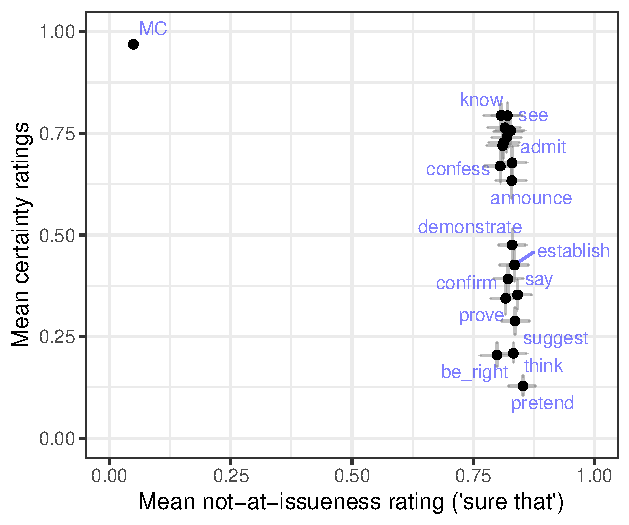
\includegraphics[scale=0.85]{figures/c1-correl.pdf}
			\caption{Mean not-at-issueness ratings vs mean certainty ratings by predicate, Exp. 1c}
			\label{fig:m1-corr}
		\end{figure}


	\subsection{2c---Conditional embedding yes, that's true+complement diagnostic (+ acceptability rating)} % (fold)
		\ex. \a. \textbf{Christopher:} If Cole discovered that Julian dances salsa, Logan will be joyful.
			\b. \textbf{Sandy:} Yes, that’s true, Julian dances salsa.
			\z.
		\z.

		\begin{figure}[h]
			\centering
			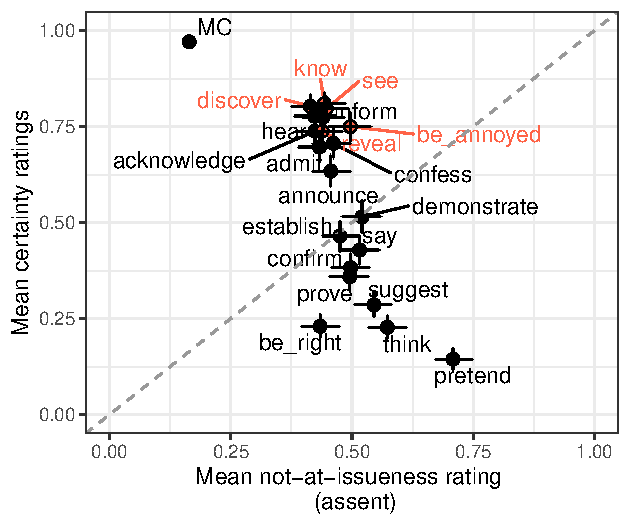
\includegraphics[scale=0.85]{figures/c2-correl.pdf}
			\caption{Mean not-at-issueness ratings vs mean certainty ratings by predicate, Exp. 2c}
			\label{fig:m1-corr}
		\end{figure}


	\subsection{3c---Conditional embedding, yes, that's true + negation of main clause (+ acceptability rating)} % (fold)
		\ex. \a. \textbf{Christopher:} If Cole discovered that Julian dances salsa, Logan will be joyful.
			\b. \textbf{Sandy:} Yes, that’s true, but Cole didn't discover it.
			\z.
		\z.

		\begin{figure}[h]
			\centering
			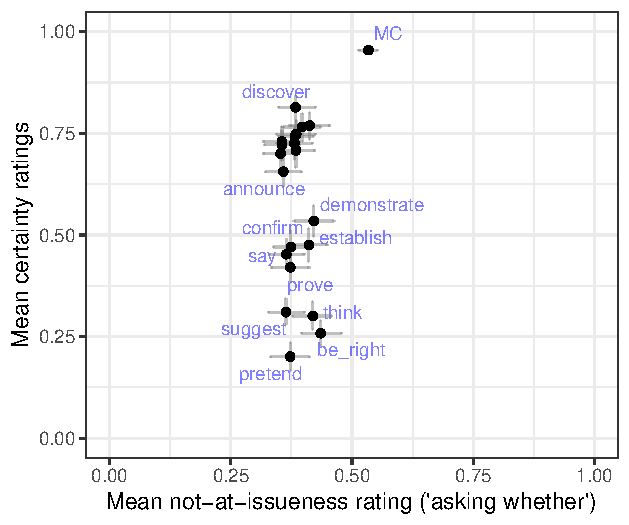
\includegraphics[scale=0.85]{figures/c3-correl.pdf}
			\caption{Mean not-at-issueness ratings vs mean certainty ratings by predicate, Exp. 3c}
			\label{fig:m1-corr}
		\end{figure}


\pagebreak
\section{To do} % (fold)
	
	\begin{itemize}
		\item 1q+2q work nicely w lexical exceptions (exceptions have to do with veridicality)
		\item What is diagnosed here?
		\item What kinds of diagnostics correspond to theories of at-issueness?
		\item Polar quesitons vs assertions as different discourse moves; also reponses to these interact with commitment in different ways
		\item Can we find a reliable diagnostic for at-issueness, about the same thing and across contexts?
		\item Aaron White and colleagues have data looking at negative inferences
		\item how do the different diagnostics and confounds w commitment shine a light on lexical differences?
	\end{itemize}

% section to_do (end)

% section today_further_questions (end)

\end{document}